%!TEX root = thesis.tex

\chapter{Visualisation Design}
\label{chap:visualisation-design}

Following the field study (see Chapter~\ref{chap:exploratory-field-study}), a strategy for visualisation prototyping and evaluation was developed. This process and the result are outlined in the following sections.

{\color{red}\cite{Ware2013a,McLean2010a,Purchase1996} will be useful here.}

\section{Rationale}



\section{Design}

\begin{figure}
  \centering 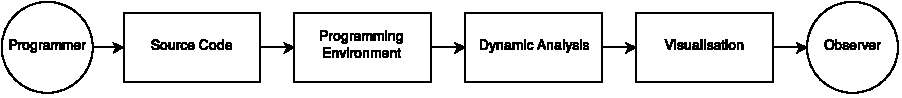
\includegraphics[width=\columnwidth]{../images/diagrams/knowledge-flow-initial.pdf}
  \caption{Knowledge flow from programmer to observer as directed by the visualisation technique employed.}
\label{fig:knowledge-flow-initial}
\end{figure}

\section{Analysis}

\section{Mappings}